\chapter{Resultados Preliminares}
\label{cap:resultados}

Neste capítulo são apresentados e analisados os resultados obtidos nessa fase do projeto, de acordo com os testes descritos anteriormente.

% --------------------------------------------------------
% ----------------- TERASORT -----------------------------
% --------------------------------------------------------
\section{\textit{Benchmarks: TeraSort} e \textit{Sort}}

A Tabela  \ref{tab:TeraSort} apresenta os resultados obtidos para o \textit{benchmark TeraSort}. Ela indica que o \textit{TeraGen} executou duas tarefas Map em 14 segundos, ou seja, esse foi o tempo utilizado pelo algoritmo para gerar dois arquivos de 50 mil linhas cada. Para ordenar os dados fornecidos pelo \textit{TeraGen}, o \textit{Terasort} executou duas tarefas Map e uma Tarefa Reduce em 22 segundos. Por fim, para validar a ordenação o \textit{TeraValidade} executou, em 22 segundos, uma tarefa Map e uma Tarefa Reduce, sem arquivos de saída, o que indica que não foram encontradas chaves fora da ordem.  

\begin{table}[htbp]
\centering
\begin{footnotesize}
\begin{tabular}{|l|c|c|c|} \hline
Algoritmo 		&Tempo (s)	 	&Tarefas Map 	&Tarefas Reduce \\ \hline \hline
TeraGen 			&14			&2					&0						\\ \hline 
TeraSort			&22			&2					&1						\\ \hline 
TeraValidade 	&22			&1					&1						\\ \hline 
\end{tabular}
\end{footnotesize}
\caption{Tempos médios do \textit{TeraSort} para ordenação em 2 máquinas}
\label{tab:TeraSort}
\end{table}

A Tabela \ref{tab:Sort} apresenta os resultados obtidos para o \textit{benchmarks} \textit{Sort} em quatro máquinas, com dez execuções cada. Para cada máquina usada na execução, foram gerados pelo \textit{RandomWriter}, dez arquivos de 1GB, em formato binário. Esses arquivos foram gerados  em 3 minutos e 54 segundos, realizando 40 tarefas Map. Para ordenar esses dados o algoritmo levou pouco mais que 37 minutos, realizando 640 tarefas Map e 7 tarefas Reduce.  

\begin{table}[htbp]
\centering
\begin{footnotesize}
\begin{tabular}{|l|c|c|c|} \hline
Algoritmo 		&Tempo (s) 	&Tarefas Map 	&Tarefas Reduce\\ \hline \hline
RandomWriter 	&234				&40					&0						\\ \hline 
Sort					&2242				&640				&7						\\ \hline 
\end{tabular}
\end{footnotesize}
\caption{Tempos médios do \textit{Sort} para ordenação em 4 máquinas}
\label{tab:Sort}
\end{table}

\section{Algoritmo Ordenação por Amostragem}

Os testes feitos com o algoritmo Ordenação por Amostragem tinham como objetivo reproduzir os resultados encontrados no trabalho feito por Pinhão (2011), e gerar resultados 
que serão utilizados posteriormente na comparação de desempenho dos algoritmos. 
O resultado dos experimentos está separado de acordo com o tipo de teste realizado, com variação do conjunto de dados, da quantidade de dados ordenada e da quantidade de máquinas utilizadas. 

% --------------------------------------------------------
% ----------------- CONSTANTE ----------------------------
% --------------------------------------------------------

\subsection{Diferentes conjuntos de dados}
Nos primeiros testes realizados com o algoritmo Ordenação por Amostragem foi mantido constante o tamanho do arquivo a ser ordenado e o número de máquinas utilizadas na ordenação. Foram usados dez conjuntos de dados diferentes, a fim de verificar se as chaves presentes no conjunto alteram o tempo de execução. 


A Tabela \ref{tab:ConjuntoTempos} apresenta a variação dos tempos das execuções da ordenação de 10$^6$ chaves em quatro máquinas. 
Esse tempo, nas diferentes distribuições, apresentou valores próximos, o que indica que a entrada de dados não gera uma variação significativa no tempo de execução do algoritmo. Isso pode ser comprovado pela Figura \ref{fig:ConjuntoTempos}, que indica ainda que a distribuição uniforme apresentou maior variação no tempo de execução: entre 37,26 segundos e 40,3 segundos.

\begin{table}[!htbp]
\centering
\begin{footnotesize}
\begin{tabular}{|C{20mm}|C{20mm}|C{20mm}|C{20mm}|C{20mm}|C{15mm}|	} \hline
\multirow{2}{*}{Distribuição} 
& \multicolumn{4}{|c|}{Tempo (s)} 
& \multirow{2}{*}{COV}  \\ \cline{2-5}
	&	Maior	&	Menor	&	Mediana	&	Média	& \\ \hline \hline
Uniforme	&	40,30	&	37,26	&	37,49	&	37,94	&	0,0236	\\ \hline
Normal	&	40,29	&	38,29	&	39,32	&	39,43	&	0,0161	\\ \hline
Pareto	&	40,28	&	38,26	&	39,32	&	39,50	&	0,0174	\\ \hline
\end{tabular}
\end{footnotesize}
\caption{Tempos médios para ordenação de 10 conjuntos de 10$^6$ dados em 4 máquinas}
\label{tab:ConjuntoTempos}
\end{table}



\begin{figure}[!htb]
\centering
%trim left, bottom, right and top
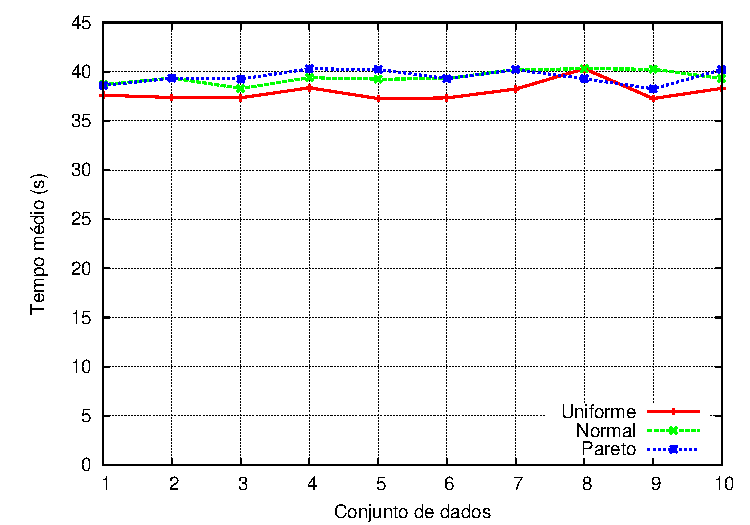
\includegraphics[width=0.75\textwidth]{figuras/ConjuntoTempo.pdf}
\caption{Gráfico dos tempos médios para ordenação de 10 conjuntos de 10$^6$ dados em 4 máquinas}
\label{fig:ConjuntoTempos}
\end{figure}

\newpage

A Tabela \ref{tab:ConjuntoParticoes} apresenta estatísticas para o número de elementos das partições nas execuções com as três distribuições. Os dados incluem média, número de elementos da maior partição, da menor e da partição mediana, resultado das dez execuções do algoritmo. 
Os valores das partições são próximos, o que indica que as cargas foram divididas de forma balanceada. 
Os coeficientes de variação são valores próximos a 0,02, o que indica pouca variação entre as maiores e as menores partições. 

\begin{table}[!htbp]
\centering
\begin{footnotesize}
\begin{tabular}{|C{20mm}|C{20mm}|C{20mm}|C{20mm}|C{20mm}|C{15mm}|	} \hline
Distribuição	&	Maior	&	Menor	&	Mediana	&	Média	&	COV	\\ \hline \hline
Uniforme	&	132024	&	118380	&	124469	&	125000	&	0,0245	\\ \hline
Normal	&	131758	&	117483	&	125634	&	125000	&	0,0235	\\ \hline
Pareto	&	133065	&	116614	&	125280	&	125000	&	0,0298	\\ \hline
\end{tabular}
\end{footnotesize}
\caption{Tamanhos médios das partições para ordenação de 10$^6$ dados em 4 máquinas}
\label{tab:ConjuntoParticoes}
\end{table}




% --------------------------------------------------------
% -------------------- DADOS -----------------------------
% --------------------------------------------------------

\subsection{Diferentes quantidades de dados}

Para avaliar a complexidade do algoritmo, foram realizados testes variando a quantidade de dados. O número de dados varia de 10$^6$ a 10$^{10}$, nas três distribuições já citadas. As ordenações foram executadas em quatro máquinas, com três execuções para cada conjunto de dados. 

A Tabela \ref{tab:QuantidadeDadosTempo} apresenta os dados para os tempos médios obtidos nas três execuções. Os tempos de execução não apresentam variações consideráveis em relação às distribuições. Observa-se que o tempo de execução de 10$^6$ dados é 39, 41 e 40 segundos nas distribuições uniforme, normal e pareto, respectivamente. Esse tempo cresce à medida que a quantidade de dados aumenta, chegando a valores próximos à 5 horas para ordenação de 10$^{10}$ dados. 

\begin{table}[htbp]
\centering
\begin{footnotesize}
\begin{tabular}{|C{17mm}|C{19mm}|m{15mm}|C{13mm}|m{15mm}|C{13mm}|m{15mm}|C{13mm}|} \hline

\multirow{3}{*}{Dados} 
& \multirow{3}{*}{\vbox{Tamanho em Bytes}} 
& \multicolumn{2}{|c|}{Uniforme}
& \multicolumn{2}{|c|}{Normal}
& \multicolumn{2}{|c|}{Pareto}

\\ \cline{3-8}
&
&Tempo Médio (s)  &COV
&Tempo Médio (s)  &COV 
&Tempo Médio (s)  &COV \\ \hline \hline

10$^6$	&	12MB	&	37	&	0,0422	&	38	&	0,0346	&	38	&	0,0567	\\ \hline
10$^7$	&	120MB	&	57	&	0,0515	&	56	&	0,0236	&	55	&	0,0121	\\ \hline
10$^8$	&	1,2GB	&	217	&	0,0243	&	219	&	0,0211	&	222	&	0,0436	\\ \hline
10$^9$	&	12GB	&	1795	&	0,0180	&	1834	&	0,0048	&	1820	&	0,0092	\\ \hline
10$^{10}$	&	120GB	&	17964	&	0,0002	&	18165	&	0,0023	&	18734	&	0,0003	\\ \hline

\end{tabular}
\caption{Tempos médios para ordenação de 10$^6$ a 10$^{10}$ dados em 4 máquinas}
\label{tab:QuantidadeDadosTempo}
\end{footnotesize}
\end{table}

A Figura \ref{fig:DadosTempo} apresenta de forma gráfica os valores de tempos médios resultantes das três execuções do algoritmo para conjuntos de dados de tamanhos 10$^6$  a 10$^{ 10}$ chaves. Nesse gráfico os eixos x e y estão em escala logarítmica para permitir melhor visualização dos dados, uma vez que os tempos médios obtidos aumentam várias ordens de grandeza à medida que a quantidade de dados aumenta.

\begin{figure}[htb]
\centering
%trim left, bottom, right and top
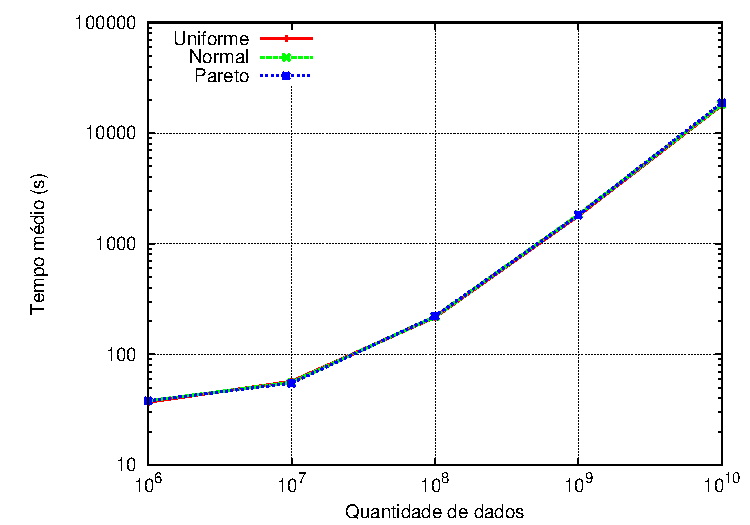
\includegraphics[width=0.75\textwidth]{figuras/DadosTempo.pdf}
\caption{Gráfico dos tempos médios para ordenação de 10$^6$ a 10$^{10}$ dados em 4 máquinas}
\label{fig:DadosTempo}
\end{figure}

Com a finalidade de dimensionar o \textit{overhead} do algoritmo, isto é, a sobrecarga ou custo adicional de comunicação entre os processadores mestre e escravos, assim como sua escalabilidade em relação ao número de dados, foi calculado o tempo médio relativo de ordenação para cada conjunto de 10$^6$ dados. 
Dessa forma, os tempos médios para ordenar 10$^7$, ou seja dez conjuntos de 10$^6$ dados foram, respectivamente, 5,7, 5,6 e 5,5 segundos para as distribuições uniforme, normal e pareto.
Já o tempo médio para ordenar dez mil conjuntos de 10$^6$  (10$^{10}$ dados) foi entre 1,79 e 1,87 segundos, o que demonstra boa escalabilidade, pois o desempenho do algoritmo aumenta com o crescimento dos dados. 
O gráfico da Figura \ref{fig:DadosOverhead} representa esses resultados. 
Pode-se observar que, à medida que a quantidade de dados para ordenação aumenta, o tempo médio para ordenação diminui. 

\begin{figure}[htb]
\centering
%trim left, bottom, right and top
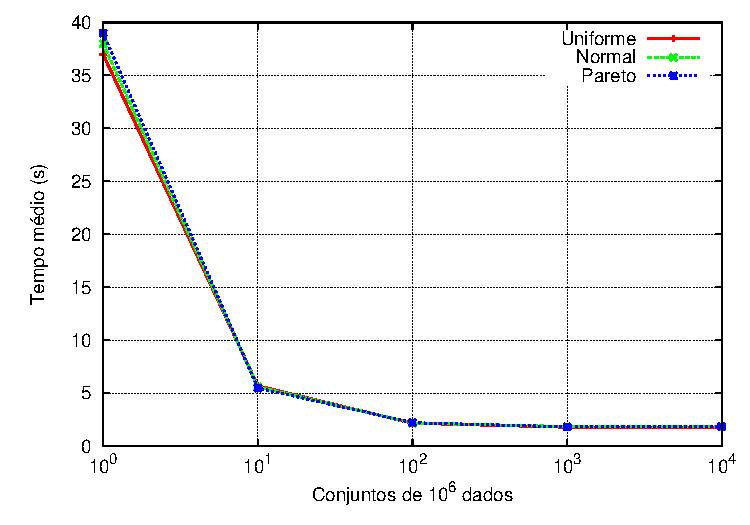
\includegraphics[width=0.75\textwidth]{figuras/DadosOverhead.pdf}
\caption{Gráfico dos tempos médios para ordenação de conjuntos de 10$^6$ dados em 4 máquinas}
\label{fig:DadosOverhead}
\end{figure}


% --------------------------------------------------------
% -------------------- MÁQUINAS --------------------------
% --------------------------------------------------------
\subsection{Diferentes quantidades de máquinas}

Foram realizados experimentos para avaliar a escalabilidade do algoritmo, a fim de se auferir o ganho de tempo que se tem com o aumento do número de máquinas. Para tanto, foram comparados além do tempo gasto em cada execução, o \textit{speedup} e a eficiência. Cada teste foi realizado três vezes, com um conjunto de 10$^8$ chaves nas distribuições normal, uniforme e pareto, em conjuntos de duas à cinco máquinas. 

A Tabela \ref{tab:QuantidadeMaquinasTempos} apresenta  os tempos gastos para as ordenações em diferentes quantidade de máquinas, nas distribuições uniforme, normal e pareto. Em geral os tempos de ordenação foram próximos nas três distribuições, sendo que a distribuição normal apresentou um tempo de execução menor em cada configuração de máquinas. 
O tempo médio para a execução em duas máquinas nas distribuições uniforme e pareto foi de pouco menos que 6 minutos e 30 segundos, e na distribuição normal foi de 6 minutos e 9 segundos. 
Três máquinas levaram aproximadamente 4 minutos e 30 segundos para concluir a ordenação. 
Com quatro máquinas o tempo de execução nas três distribuições são próximos ou iguais a 3,5minutos. 
Em cinco máquinas a execução da ordenação foi realizada em aproximadamente 3 minutos. 
Os coeficientes de variação encontrados foram pequenos, o que indica pequena variação entre os tempos de execução.


\begin{table}[htbp]
\centering
\begin{footnotesize}
\begin{tabular}{|C{15mm}|C{16mm}|C{14mm}|C{16mm}|C{14mm}|C{16mm}|C{14mm}|} \hline

\multirow{3}{*}{Máquinas} 
& \multicolumn{2}{|c|}{Uniforme}
& \multicolumn{2}{|c|}{Normal}
& \multicolumn{2}{|c|}{Pareto}
\\ \cline{2-7}
&Tempo Médio (s)  &COV
&Tempo Médio (s)  &COV 
&Tempo Médio (s)  &COV \\ \hline \hline

2	&	384	&	0,0023	&	370	&	0,0067	&	382	&	0,0053	\\ \hline
3	&	264	&	0,0030	&	258	&	0,0114	&	382	&	0,0030	\\ \hline
4	&	213	&	0,0095	&	208	&	0,0012	&	210	&	0,0020	\\ \hline
5	&	177	&	0,0081	&	173	&	0,0058	&	178	&	0,0003	\\ \hline
\end{tabular}
\end{footnotesize}
\caption{Tempos médios para ordenação de 10$^8$ dados em de 2 a 5 máquinas}
\label{tab:QuantidadeMaquinasTempos}
\end{table}

\begin{figure}[!htb]
\centering
%trim left, bottom, right and top
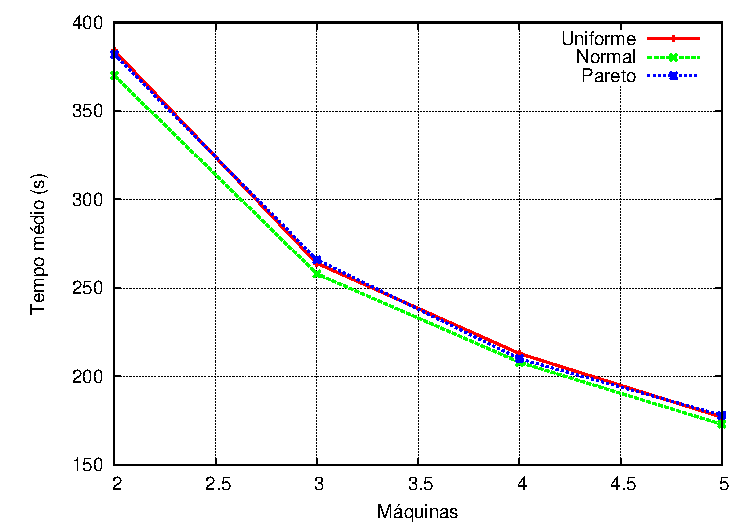
\includegraphics[width=0.75\textwidth]{figuras/MaquinasTempo.pdf}
\caption{Tempos médios para ordenação de 10$^8$ dados em de 2 a 5 máquinas}
\label{fig:MaquinasTempos}
\end{figure}

A Figura \ref{fig:MaquinasTempos} representa graficamente a variação do tempo à medida que o número de máquinas aumenta. Como se pode observar essa variação é bem próxima para as três distribuições. Ainda pode-se observar que a diminuição do tempo não é exatamente linear, ou seja, não ocorre na mesma proporção em que o número de máquinas aumenta. 



A fim de avaliar o desempenho do algoritmo em diferentes configurações de máquinas e nas três distribuições foram avaliadas as métricas \textit{speedup} e eficiência. % , conforme representado nas Tabelas  e \ref{tab:QuantidadeDadosEficiencia} respectivamente. 
Como foi descrito na seção \ref{sec:computacaoparalela} o \textit{speedup} indica quão mais rápida é a aplicação paralela comparada à aplicação sequencial. Já a eficiência  indica a taxa de utilização de cada processador. Ela é  excelente quando é 100\% indicando que os processadores tem utilização total.
Nesse trabalho o algoritmo foi implementado apenas em paralelo, assim, considera-se para fins de comparação a execução em apenas dois computadores como a implementação de referência. As fórmulas foram adaptadas para verificar a melhora de desempenho e eficiência obtidas a partir de duas máquinas: 
\[ Sp = \frac{T_{4 processadores}}{T_{paralelo}}    \hspace*{3cm}  E = \frac{Sp_{real}}{Sp_{ideal}}\]

Observa-se na Tabela \ref{tab:QuantidadeDadosSpeedup} que à medida que aumenta o número de processadores o \textit{speedup} real se afasta do \textit{speedup} ideal. Assim temos em uma máquina o mesmo \textit{speedup} ideal e real, e em 5 máquinas e 10 processadores o \textit{speedup} real é em torno de 85\% do \textit{speedup} ideal. A variação do \textit{speedup} já era um comportamento esperado, uma vez que paralelizações em geral introduzem sobrecargas para realizar o balanceamento e a comunicação entre os processos.


\begin{table}[htbp]
\centering
\begin{footnotesize}
\begin{tabular}{|C{20mm}|p{12mm}|p{14mm}|p{12mm}|p{14mm}|p{12mm}|p{14mm}|p{13mm}|} \hline

\multirow{2}{*}{Processadores} 
& \multicolumn{2}{|c|}{Uniforme}
& \multicolumn{2}{|c|}{Normal}
& \multicolumn{2}{|c|}{Pareto}
& Speedup
\\ \cline{2-7} 
&Tempo Médio (s) &Speedup Real
&Tempo Médio (s)  &Speedup Real
&Tempo Médio (s)  &Speedup Real
&Ideal \\ \hline \hline
 
4		&	384	&	1	&	370	&	1	&	382	&	1	&	1	\\ \hline
6		&	264	&	1,4534	&	258	&	1,4341	&	266	&	1,4361	&	1,5	\\ \hline
8		&	213	&	1,8010	&	208	&	1,7788	&	210	&	1,8190	&	2	\\ \hline
10		&	177	&	2,1732	&	173	&	2,1387	&	178	&	2,1461	&	2,5	\\ \hline

\end{tabular}
\end{footnotesize}
\caption{Resultados do \textit{speedup} para execuções de 4 a 10 processadores}
\label{tab:QuantidadeDadosSpeedup}
\end{table}

A Figura \ref{fig:MaquinasSpeedup} apresenta o crescimento do \textit{speedup} real à medida que o número de processadores aumenta e  o \textit{speedup} ideal para comparação. Como se pode ver, inicialmente ambos valores de \textit{speedup} são iguais, mas com o aumento no número de processadores a curva representando o valor do \textit{speedup} real se afasta da curva do \textit{speedup} ideal, fato que ocorre nas três distribuições.

\begin{figure}[htb]
\centering
%trim left, bottom, right and top
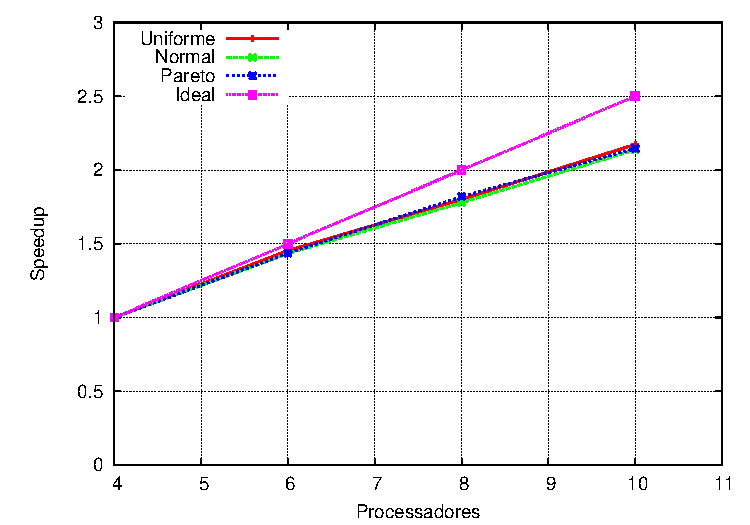
\includegraphics[width=0.75\textwidth]{figuras/MaquinasSpeedup.pdf}
\caption{Gráfico dos resultados do \textit{speedup} para execuções de 4 a 10 processadores}
\label{fig:MaquinasSpeedup}
\end{figure}


A Tabela \ref{tab:QuantidadeDadosEficiencia} apresenta os valores de eficiência calculados para as diferentes quantidades de processadores utilizados na ordenação. Observa-se que conforme aumenta a quantidade de processadores o valor da eficiência decresce, mostrando que com maior número de processadores, estes possuem uma taxa de utilização menor. Contudo, o percentual de eficiência é sempre próximo do máximo, o que indica uma boa escalabilidade do algoritmo. Além disso, observa-se que a eficiência não sofre influência significativa da distribuição do conjunto de dados.

\begin{table}[htbp]
\centering
\begin{footnotesize}
\begin{tabular}{|C{25mm}|C{25mm}|C{25mm}|C{25mm}|} \hline

\multirow{2}{*}{Processadores} 
& Uniforme
& Normal
& Pareto
\\ \cline{2-4} 
&Eficiência(\%)  &Eficiência(\%) &Eficiência(\%) 
\\ \hline \hline
%processadores 	Uniforme 		Normal 		Pareto 
%							Eficiência(%)
4		&	100	&	100	&	100		\\ \hline
6		&	96,90	&	95,61	&	95,74		\\ \hline
8		&	90,05	&	88,94	&	90,95		\\ \hline
10		&	86,93	&	85,55	&	85,84		\\ \hline
\end{tabular}
\end{footnotesize}
\caption{Resultados da eficiência para execuções de 4 a 10 processadores}
\label{tab:QuantidadeDadosEficiencia}
\end{table}

A Figura \ref{fig:MaquinasEficiencia} representa graficamente a eficiência em diferentes números de processadores. Nela observa-se que à medida que o número de processadores aumenta o percentual da eficiência diminui. Percebe-se ainda que a distribuição normal apresenta menores valores em todas as configurações de processadores.

\begin{figure}[htb]
\centering
%trim left, bottom, right and top
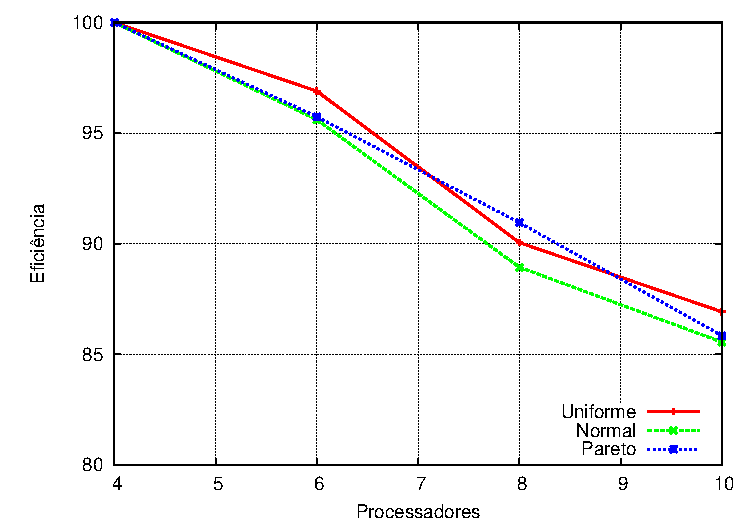
\includegraphics[width=0.75\textwidth]{figuras/MaquinasEficiencia.pdf}
\caption{Gráfico dos resultados da eficiência para execuções de 4 a 10 processadores}
\label{fig:MaquinasEficiencia}
\end{figure}

%\subsection{Considerações Finais}
